\chapter{Implementacja}
\label{cha:rozdz4}

W tym rozdziale opisuję wymagania wobec projektu, który zawiera implementację gry ,,Love Letter'' i opisanych algorytmów. Następnie przedstawiam koncepcję wykonania wraz z diagramami UML, a na końcu prezentuję system i opisuję problemy napotkane w trakcie realizacji.

\section{Analiza wymagań}
Ponieważ celem pracy jest porównanie działania algorytmów gry karcianej, pierwszym krokiem potrzebnym do jego realizacji jest zaimplementowanie samej gry. Jak zostało to napisane w [\ref{bib:analiza_wymagan}], przed właściwą implementacją programu należy określić jego wymagania funkcjonalne i niefunkcjonalne. Większość wymagań jest już udokumentowana w postaci zasad gry opisanych w rozdziale \ref{cha:rozdz2}, należy jednak wyszczególnić pewne dodatkowe wymogi:
\begin{itemize}
	\item program musi udostępniać interfejs do którego można podłączyć różne algorytmy podejmujące decyzje,
	\item interfejs musi udostępniać aktualny stan gry oraz zbiór decyzji możliwych do podjęcia,
	\item interfejs musi zawierać funkcjonalność pozwalającą na utworzenie nowej instancji gry z zadanym stanem początkowym i podjętą decyzją. W nowej instancji wszystkie nieznane elementy gry są losowane na nowo (np. talia karta jest przetasowywana),
	\item program musi umożliwiać wybranie dwóch dowolnych algorytmów, które będą ze sobą grać, oraz ustawienie liczby gier które rozegrają,
	\item algorytm MCTS powinien mieć możliwość ustawienia dwóch parametrów: czasu wykonania, oraz algorytmu przeciwnika wykorzystywanego w symulacjach,
	\item po skończonej serii gier program powinien wyświetlać szczegółowe statystyki rozgrywek w formie wykresu i zapisywać dane do pliku.
\end{itemize}
Do zwracanych statystyk powinny należeć:
\begin{itemize}
	\item procentowa liczba zwycięstw każdego algorytmu z wyszczególnieniem na tury w których została zakończona runda.
	\item rozkład procentowy zakończeń gry - ile rund skończyło się zagraniem karty Barona, Strażniczki, Księcia lub w ostatniej turze po wyczerpaniu talii.
	\item wyszczególnienie procentowej liczby zwycięstw w zależności od tego który algorytm wykonuje ruch jako pierwszy.
\end{itemize}

Wymagania niefunkcjonalne:
\begin{itemize}
	\item program powinien uruchamiać się bez względu na środowisko.
	\item program nie powinien wymagać od użytkownika znajomości szczegółów implementacji.
	\item program powinien udostępniać instrukcje pomocy.
	\item aplikacja powinna zostać zaprojektowana w taki sposób, żeby można było dodawać kolejne algorytmy do aplikacji bez konieczności modyfikacji kodu
\end{itemize}
\clearpage
1	
\section{Koncepcja wykonania i wykorzystane technologie}
By skupić się wyłączne na merytorycznym działaniu projektu, postanowiłem zaimplementować program w postaci aplikacji konsolowej, gdzie komunikacja odbywa się za pomocą wiersza poleceń$^{[\ref{bib:wiki_wierszPolecen}]}$. Wprowadzenie warstwy graficznej jest zbędne wobec postawionych wymagań.

Pomimo prostoty i niezmienności wymagań funkcjonalnych, projekt zostanie wykonany zgodnie z metodyką zwinną (ang. agile methodology)$^{[\ref{bib:wiki_waterfall}]}$, która wciąż zyskuje na popularności względem metodyk kaskadowych. Jej główną cechą jest porzucenie szczegółowego planowania projektu na rzecz obserwacji i reagowania. Całość oprogramowania jest wytwarzana w kolejnych iteracjach, w których implementowane są kolejne funkcjonalności, oraz testowane i poprawiane wcześniejsze. Poniżej prezentuję zaplanowane przeze mnie iteracje tworzenia projektu(Rys. \ref{fig:diagramIteracji}.):

\begin{figure}[H]
	\centering
	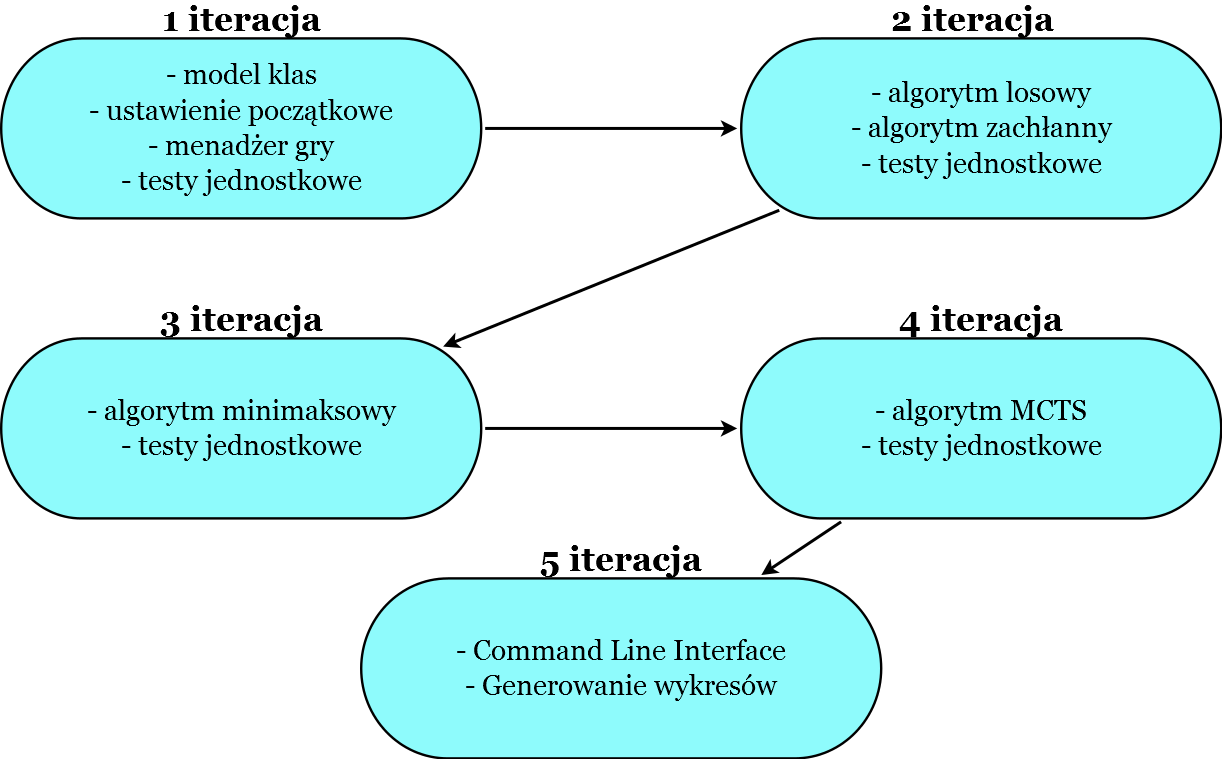
\includegraphics[width=\textwidth]{Resources/DiagramIteracji.png}
	\caption{Zaplanowane iteracje} 
	\label{fig:diagramIteracji}
\end{figure}

Ze względu na osobiste umiejętności, do implementacji wybrałem język programowania Java SE w wersji 8$^{[\ref{bib:java}]}$. Jest to język obiektowy, o ścisłym typowaniu, działający na maszynie wirtualnej Javy, co zapewnia kompatybilność ze wszystkimi systemami operacyjnymi. Całość projektu wykonałem w środowisku programistycznym IntelliJ IDEA w darmowej wersji Community$^{[\ref{bib:intellij}]}$.

\section{Diagramy}
Poniżej prezentuję diagramy klas UML, dokumentujące obecną strukturę kodu. 
\subsection{Diagram klas pakietu model}

\begin{figure}[H]
	\centering
	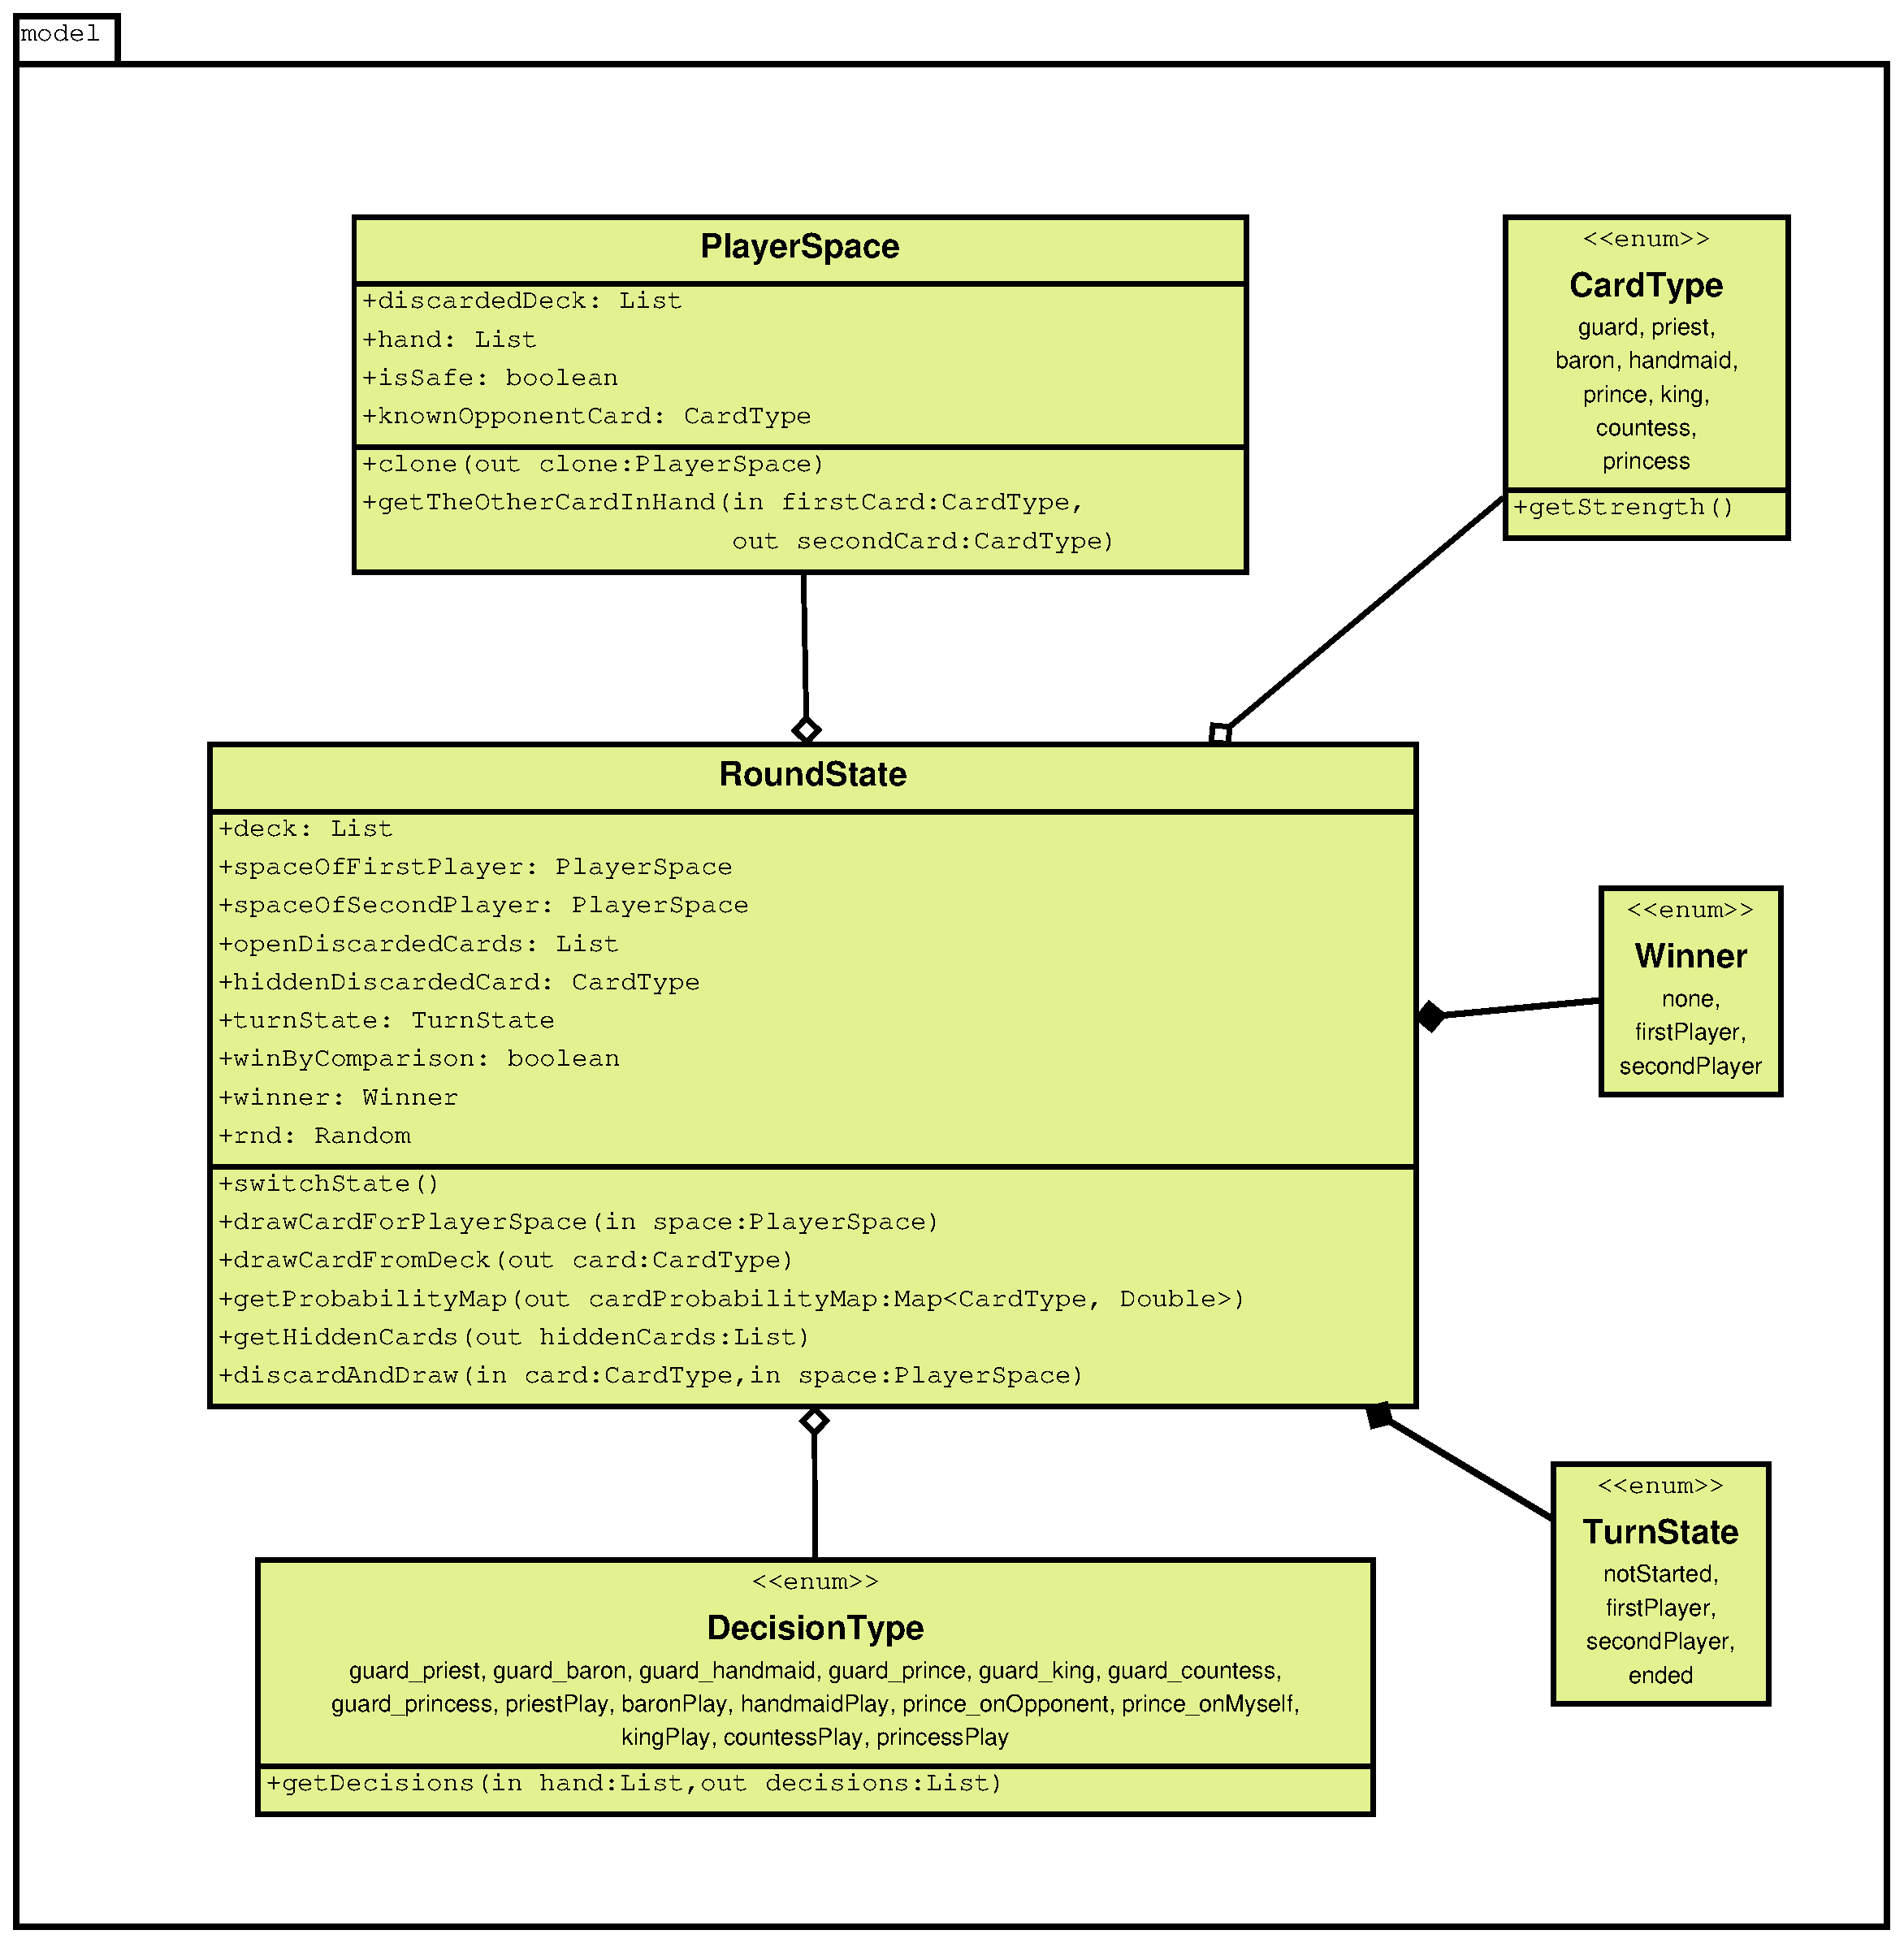
\includegraphics[width=\textwidth]{Resources/diagramKlas_model.eps}
	\caption{Diagram klas pakietu \textit{model}} 
	\label{fig:diagramKlasModel}
\end{figure}

W danym pakiecie znajdują się wszystkie elementy składające się na samą grę. Głównym element jest klasa RoundState, odpowiadająca wierzchołkom $s_i$ należącym do zbioru $S$. Karty oraz wynikające z nich decyzje utworzone reprezentowane są w postaci klas typu enum.

\subsection{Diagram klas pakietu player}

\begin{figure}[H]
	\centering
	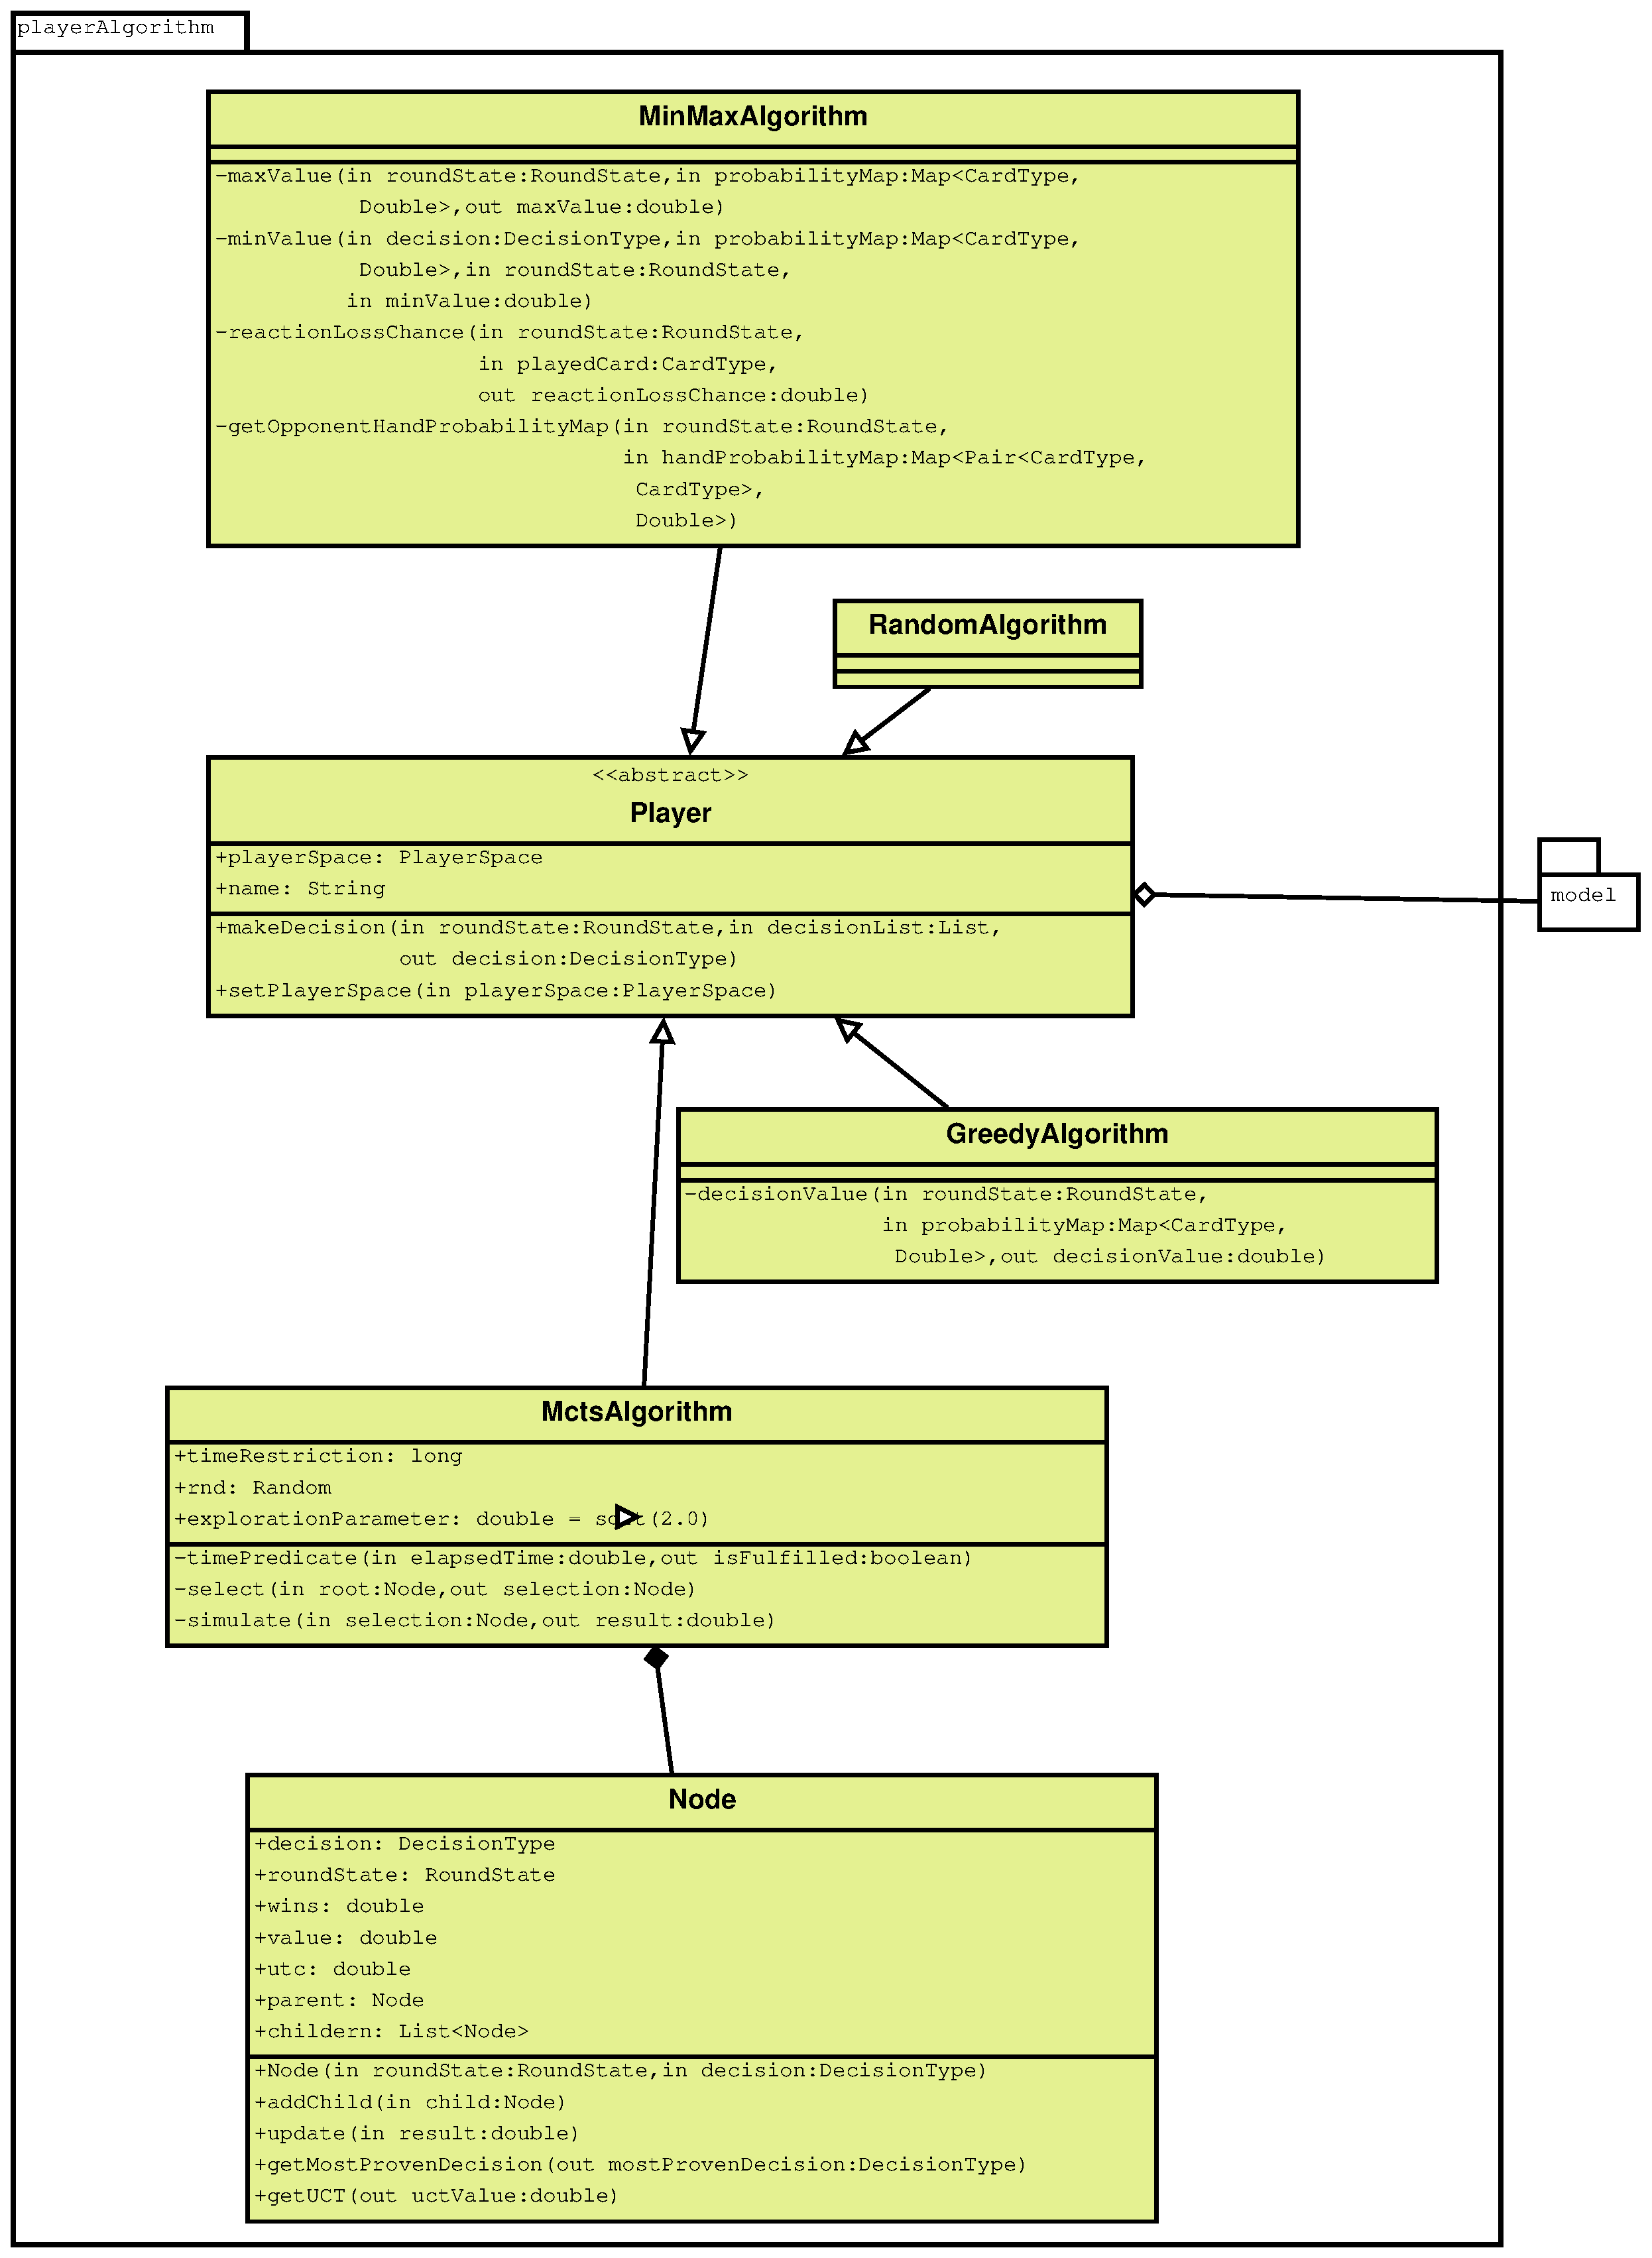
\includegraphics[width=\textwidth]{Resources/diagramKlas_player.eps}
	\caption{Diagram klas pakietu \textit{player}} 
	\label{fig:diagramKlasPlayer}
\end{figure}

W tym pakiecie głównym elementem jest klasa abstrakcyjna Player, po której dziedziczą implementowane przeze mnie algorytmy. Warto zauważyć, że wykorzystuje również pakiet \textit{model}. Takie polimorficzne rozwiązanie znacznie ułatwia dodawanie kolejnych algorytmów do aplikacji, bez konieczności modyfikowania jej.

\subsection{Diagram klas pakietu engine}

\begin{figure}[H]
	\centering
	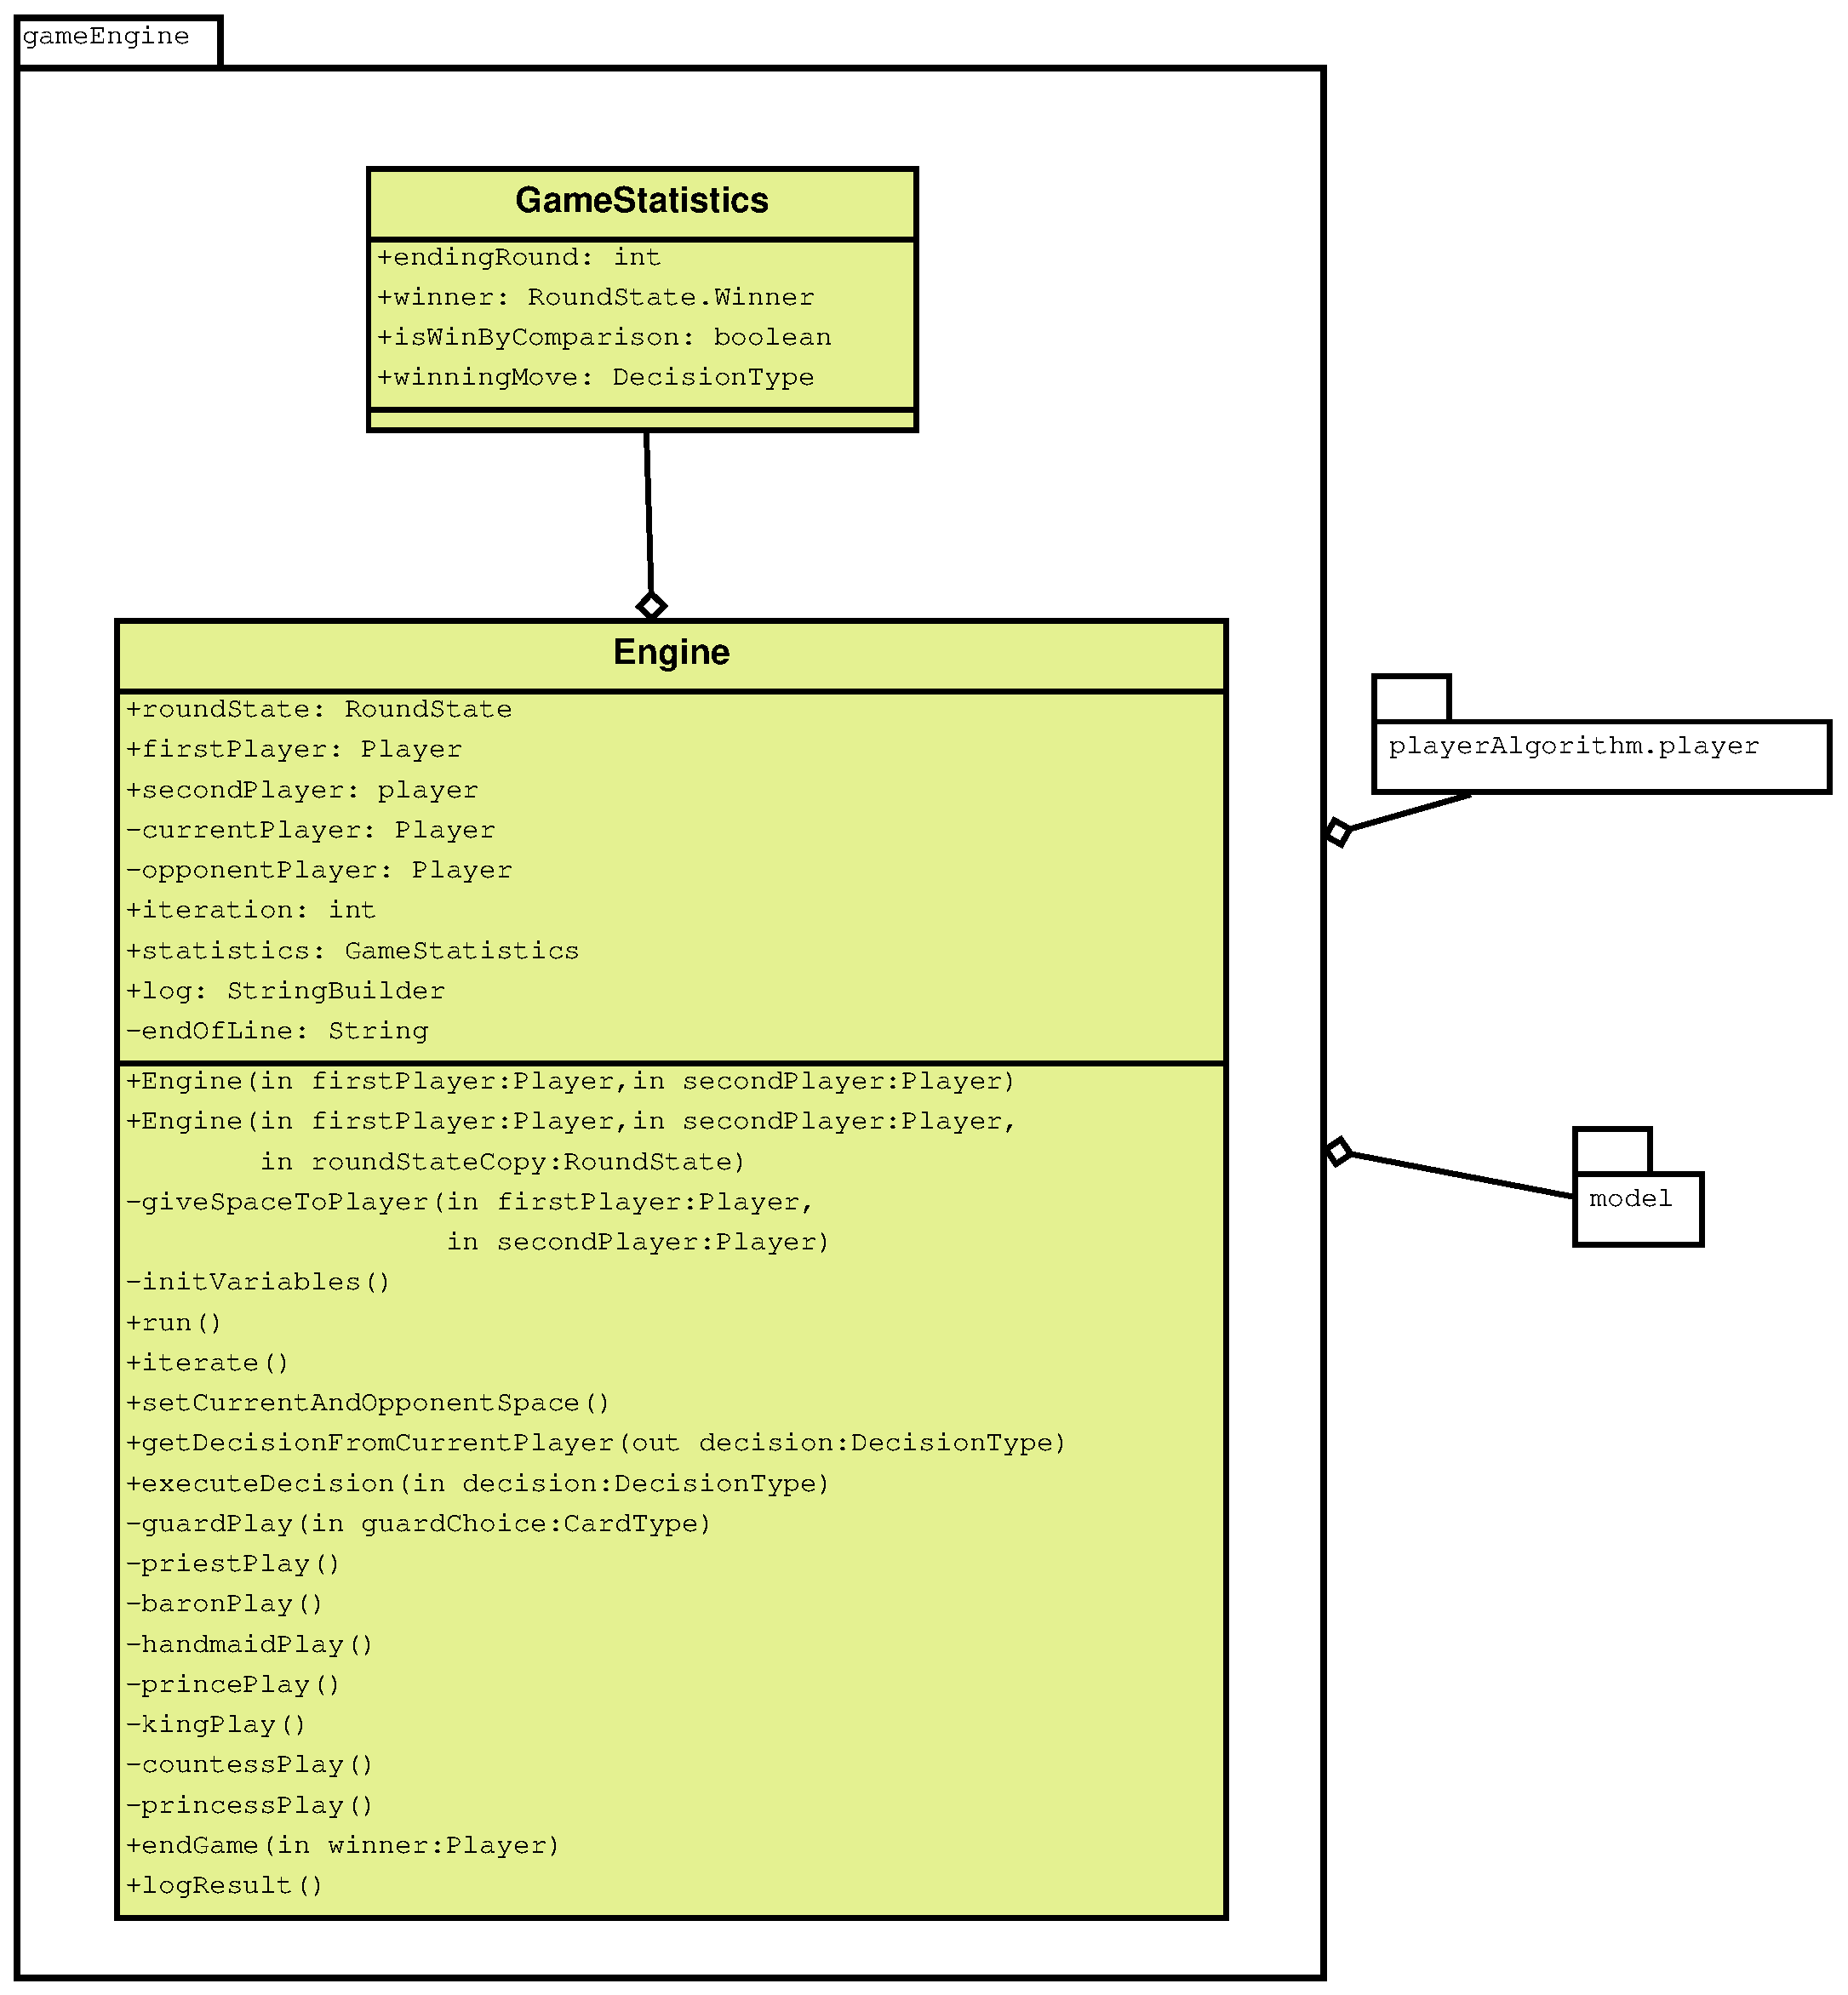
\includegraphics[width=\textwidth]{Resources/diagramKlas_engine.eps}
	\caption{Diagram klas pakietu \textit{gameEngine}} 
	\label{fig:diagramKlasEngine}
\end{figure}
Ten pakiet realizuje zasady gry w sensie mechaniki działania kart. Klasa \textit{Engine} jest menadżerem i zarządza stanem gry na podstawie decyzji otrzymanej z klasy \textit{Player}. Metoda \textit{giveSpaceToPlayer} przekazuje obiektom klasy \textit{Player} referencję do \textit{PlayerSpace} i kopię obiektu \textit{RoundState}. 


\section{Listingi}
Pisząc kod aplikacji, oprócz kierowania się paradygmatami programowania obiektowego, bardzo ważne jest również by dbać o czytelność kodu. W [\ref{bib:czysty_kod}] można znaleźć wiele porad i metod zwiększających jakość kodu. Jak taki kod powinien wyglądać bardzo dobrze opisuje Grady Booch:
\begin{center}
	,,Czysty kod jest prosty i bezpośredni. Czysty kod czyta się jak dobrze napisaną prozę. Czysty kod nigdy nie zaciemnia zamiarów projektanta; jest pełen abstrakcji i prostych ścieżek sterowania.''$^{[\ref{bib:czysty_kod_cytat_booch}]}$
\end{center}
Najpopularniejszą metodologią wspomagającą tworzenie czystego kodu jest SOLID. Jest to mnemonik opisujący pięć podstawowych założeń programownia obiektowego$^{[\ref{bib:wiki_SOLID}]}$. SOLID oznacza:
\begin{itemize}
	\item S (Single responsibility principle) - Klasa powinna posiadać jedną odpowiedzialność
	\item O (Open/closed principle) - Zmiana wymagań wobec aplikacji nie powinna w konsekwencji zmieniać kodu, lecz dodawać nowe funkcjonalności bez usuwania starych.
	\item L (Liskov substitution principle) - W przypadku dziedziczenia, klasy pochodne muszą mieć możliwość realizacji funkcji klasy bazowej.
	\item I (Interface segregation principle) - Klient nie może być uzależniony od nieużywanego przez niego interfejsu.
	\item D (Dependency inversion principle) - Funkcjonalność wysokopoziomowych modułów nie może zależeć od sposobu działania modułów niskopoziomowych.
\end{itemize}

\subsection{Listing części metod klasy Engine}
\begin{lstlisting}[language=java,label=lst:engine,caption=Część metod klasy Engine, breaklines=true]
public void run(){
    do{
	    iterate();
    }while(roundState.turnState != RoundState.TurnState.ended);
    logResult();
}
    
public void iterate(){
    setCurrentAndOpponentSpace();
    roundState.drawCardForPlayerSpace(currentPlayer.playerSpace);
    
    DecisionType decision;
    decision = getDecisionFromCurrentPlayer();
    executeDecision(decision);
    
    
    statistics.winningMove = decision;
    if( roundState.deck.size() == 0 && roundState.turnState != RoundState.TurnState.ended){
	    endGame(null);
	    return;
    }
    roundState.switchState();
    iteration++;
}
    
public DecisionType getDecisionFromCurrentPlayer(){
    return currentPlayer.makeDecision(new RoundState(roundState, currentPlayer.playerSpace), DecisionType.getDecisions(currentPlayer.playerSpace.hand));
}
        
\end{lstlisting}

\subsection{Listing algorytmu MCTS}

\begin{lstlisting}[language=java,label=lst:node,caption=Klasa Node, breaklines=true]
class Node{
	DecisionType decision;
	RoundState roundState;
	double wins;
	double value;
	double visits;
	double utc;
	Node parent;
	List<Node> children;
	
	Node(RoundState roundState, DecisionType decision){
		this.decision = decision;
		this.roundState = roundState;
		wins = 0;
		value = 0.0;
		visits = 0;
		parent = null;
		children = new ArrayList<>();
	}
	
	public void addChild(Node child){
		children.add(child);
		child.parent=this;
	}
	
	public void update(double result){
		visits++;
		wins +=result;
		value = wins/visits;
		if( visits == 0 || parent == null )
			utc = -1;
		else
			utc =  value/visits + explorationParameter * Math.sqrt( Math.log( parent.visits ) / visits);
	}
	
	public DecisionType getMostProvenDecision(){
		Node mostProvenChild = children.get(0);
		for( Node child : children ){
			if( child.visits > mostProvenChild.visits)
				mostProvenChild = child;
		}
		
		return mostProvenChild.decision;
	}
	
	private double getUCT() {
		if( visits == 0 )
			return 1000 + rnd.nextInt(20);
		return value/visits + explorationParameter * Math.sqrt( Math.log( parent.visits ) / visits);
	}
}

\end{lstlisting}

\begin{lstlisting}[language=java,label=lst:mcts,caption=Wybrane metody klasy MctsAlgorithm, breaklines=true]
@Override
public DecisionType makeDecision(RoundState roundState, List<DecisionType> decisionList) {
	Node root = new Node( new RoundState(roundState, playerSpace), null );
	
	long startTime = System.currentTimeMillis();
	long elapsedTime;
	int iteration = 0;
	boolean shouldContinue = true;
	do{
		Node selectedNode = select(root);
		if( selectedNode.roundState.turnState != RoundState.TurnState.ended ) {
			List<DecisionType> selectionDecisionList = DecisionType.getDecisions(selectedNode.roundState.spaceOfFirstPlayer.hand);
			for (DecisionType decision : selectionDecisionList) {
				selectedNode.addChild(new Node(new RoundState(roundState, roundState.spaceOfFirstPlayer), decision));
			}
			Node child = selectedNode.children.get(rnd.nextInt(selectedNode.children.size()));
			double result = simulate(child);
			do {
				child.update(result);
				child = child.parent;
			} while (child != null);
		}
		elapsedTime = System.currentTimeMillis() - startTime;
		iteration++;
	}while (timePredicate(elapsedTime));
	
	DecisionType mostProvenDecision = root.getMostProvenDecision();
	return mostProvenDecision;
}
    
private Node select(Node node) {
	if( node.children.size() == 0  ){
		return node;
	}
	
	Node selection = node.children.get(0);
	Map<DecisionType, Double> utcMap = new HashMap<>();
	for( Node child : node.children ){
		if( child.getUCT() > selection.getUCT() || selection.getUCT() == 0 )
			selection = child;
		utcMap.put(child.decision, child.getUCT());
	}
	return select(selection);
}

\end{lstlisting}

\section{Prezentacja systemu}
Poniższe zrzuty ekranu prezentują trzy widoki aplikacji: widok główny (początkowy), przebieg pojedynczej gry oraz podczas prezentacji wyników symulacji.
\subsection*{Widok główny}
\begin{figure}[H]
	\centering
	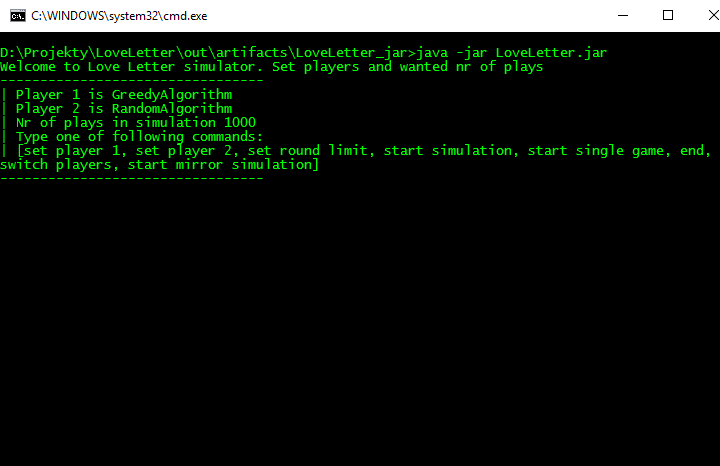
\includegraphics[width=\textwidth]{Resources/cli.PNG}
	\caption{Widok główny aplikacji} 
	\label{fig:cli}
\end{figure}
Powyższy zrzut prezentuje menu aplikacji, w którym można wpisywać odpowiednie komendy.

\subsection*{Widok ustawień i gry}
\begin{figure}[H]
	\centering
	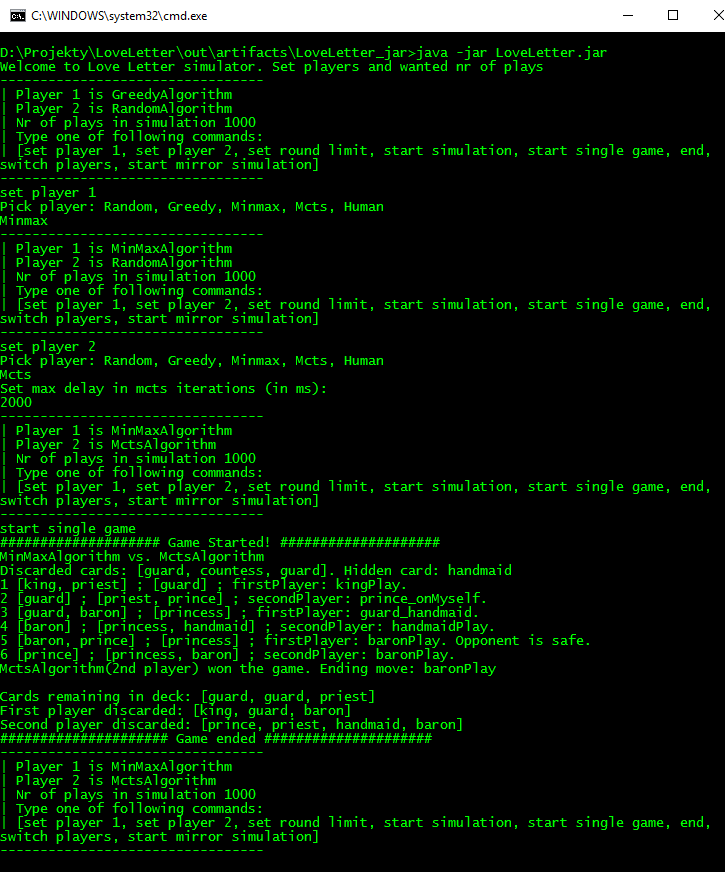
\includegraphics[width=\textwidth]{Resources/cli2.PNG}
	\caption{Widok główny aplikacji} 
	\label{fig:cli2}
\end{figure}

Na powyższym zrzucie można zauważyć ustawianie algorytmu dla gracza pierwszego i drugiego oraz przebieg pojedynczej gry. Na początku znajduje się informacja które algorytmy ze sobą grają, następnie jakie karty zostały odrzucone w układzie początkowym, a potem przebieg w następującej postaci:
\begin{center}
	[numer rundy] [karty pierwszego gracza] ; [karty drugiego gracza] ; [czyj ruch]: [podjęta decyzja]
\end{center}
Na końcu wskazany jest zwycięski algorytm, ruch kończący, oraz stosy kart odrzuconych.

\subsection*{Wykresy symulacji}
\begin{figure}[H]
	\centering
	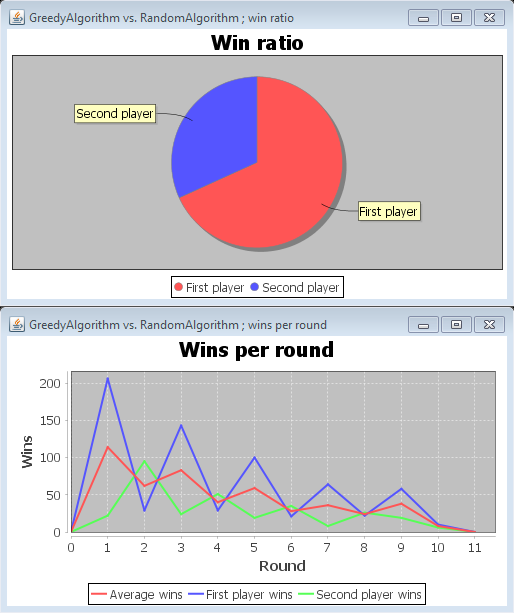
\includegraphics[]{Resources/winCharts.PNG}
	\caption{Widok główny aplikacji} 
	\label{fig:winChart}
\end{figure}

Na powyższym wykresie wskazany jest stosunek zwycięstw na wykresie kołowym, oraz ilość zwycięstw każdego z algorytmów w danej rundzie, z uwzględnieniem średniej.

\begin{figure}[H]
	\centering
	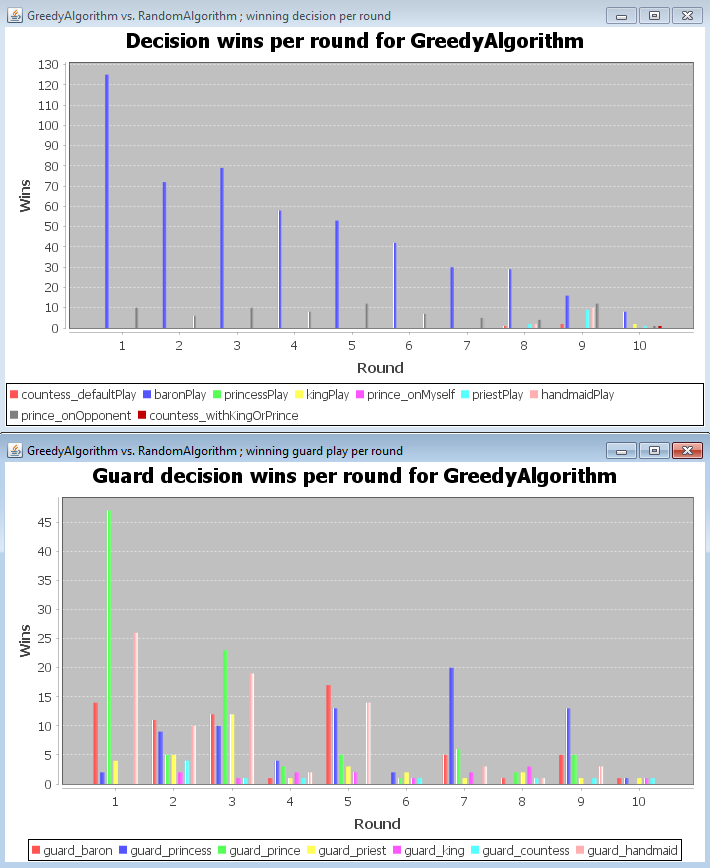
\includegraphics[width=\textwidth]{Resources/decisionWinsPerRoundChart.PNG}
	\caption{Widok główny aplikacji} 
	\label{fig:decisionChart}
\end{figure}

Powyższe wykresy słupkowe prezentują rozkład wygrywających decyzji danego gracza w zależności od rundy.

\section{Problemy napotkane w trakcie realizacji}
Jednym z problemów w aplikacji jest bardzo duża ilość instrukcji \textit{switch}. Wynika to z błędnie przyjętego modelu odwzorowania dostępnych decyzji w postaci klasy \textit{Enum}. Zdecydowanie lepszym rozwiązaniem byłoby utworzenie hierarchii klas odpowiadających każdej decyzji, które dziedziczyłyby po jednej wspólnej klasie, np. \textit{Play}. Takie podejście znacznie zredukowałoby ilość niepotrzebnego kodu i zwiększyło jego czytelność.

Kolejną rzeczą sprawiającą wiele problemów jest kwestia interfejsu \textit{Copy} w Javie. Podczas testów przesyłania kopii stanu rundy do algorytmu podejmującego decyzje powstawało wiele problemów z kopiowaniem referencji, wobec czego postanowiłem ręcznie napisać metodę kopiującą.

Ze względu na dużą ilość losowanych parametrów, trudność sprawiło napisanie odpowiednich testów pokrywających wszystkie przypadki. W związku z tym testy sprawdzające fragmenty związane z losowaniem uruchamiana są wielokrotnie. Co prawda takie podejście sprawia, że nigdy nie mamy 100\% pewności przejścia wszystkich testów bez zmiany kodu, natomiast pozwala wykryć znacznie większą ilość przypadków brzegowych, które normalnie nie były by pokryte testem.